\documentclass[border=14pt,tikz]{standalone}
\usepackage{fontspec}
\setmainfont{Helvetica Neue}
\setsansfont{Helvetica Neue}
\setmonofont{Menlo}
\usepackage{tikz}
\usetikzlibrary{positioning, arrows.meta, fit, backgrounds}

\definecolor{pure}{HTML}{E8F5E9}
\definecolor{pureborder}{HTML}{4CAF50}
\definecolor{impure}{HTML}{FFF3E0}
\definecolor{impureborder}{HTML}{FF9800}
\definecolor{model}{HTML}{E3F2FD}
\definecolor{modelborder}{HTML}{2196F3}

\begin{document}
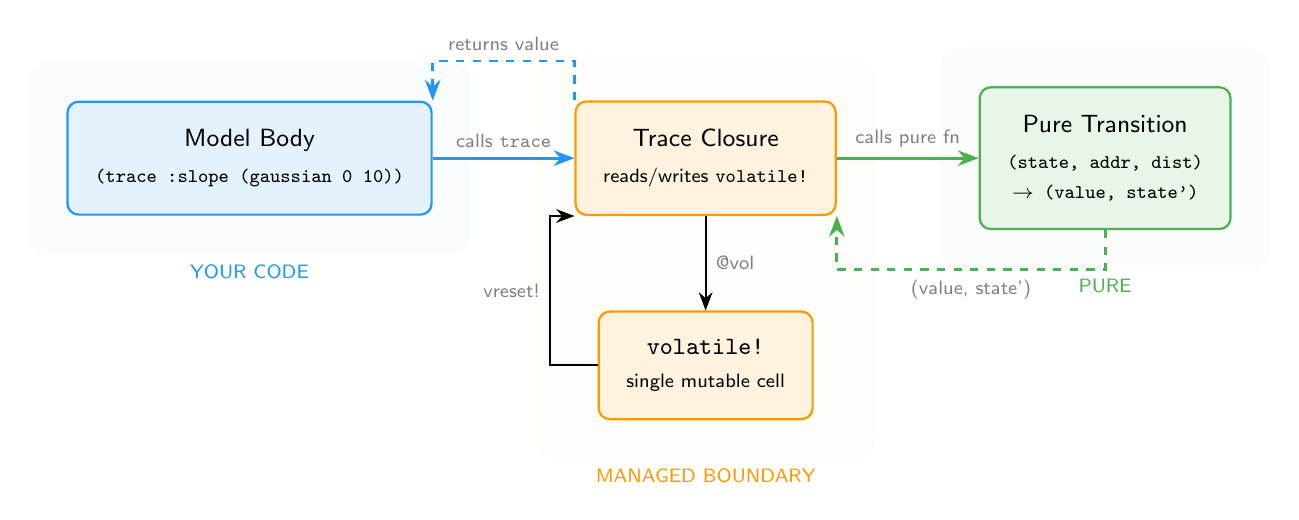
\begin{tikzpicture}[
    >=Stealth,
    node distance=1.8cm,
    box/.style={draw, rounded corners=4pt, inner sep=10pt,
                font=\sffamily\small, align=center, line width=0.8pt},
    annot/.style={font=\sffamily\scriptsize, text=black!50},
]

% Three main boxes in a row
\node[box, fill=model, draw=modelborder]
    (model) {Model Body\\[2pt]{\ttfamily\scriptsize (trace :slope (gaussian 0 10))}};

\node[box, fill=impure, draw=impureborder, right=of model]
    (closure) {Trace Closure\\[2pt]{\scriptsize reads/writes \texttt{volatile!}}};

\node[box, fill=pure, draw=pureborder, right=of closure]
    (transition) {Pure Transition\\[2pt]{\ttfamily\scriptsize (state, addr, dist)}\\{\ttfamily\scriptsize $\to$ (value, state')}};

% volatile! below closure
\node[box, fill=impure, draw=impureborder, below=1.2cm of closure]
    (vol) {\texttt{volatile!}\\[1pt]{\scriptsize single mutable cell}};

% Forward arrows (top path)
\draw[->, line width=1pt, modelborder]
    (model) -- (closure) node[midway, above, annot] {calls \texttt{trace}};
\draw[->, line width=1pt, pureborder]
    (closure) -- (transition) node[midway, above, annot] {calls pure fn};

% Return arrows (bottom path, using bend)
\draw[->, line width=1pt, pureborder, dashed]
    (transition.south) -- ++(0,-0.5) -| (closure.south east)
    node[pos=0.25, below, annot] {(value, state')};
\draw[->, line width=1pt, modelborder, dashed]
    (closure.north west) -- ++(0,0.5) -| (model.north east)
    node[pos=0.25, above, annot] {returns value};

% Closure <-> volatile
\draw[->, line width=0.8pt] (closure) -- (vol) node[midway, right, annot] {@vol};
\draw[->, line width=0.8pt] (vol.west) -- ++(-.6,0) |- (closure.south west)
    node[pos=0.25, left, annot] {vreset!};

% Background zones via fit
\begin{scope}[on background layer]
    \node[fit=(model), fill=model!20, rounded corners=8pt, inner sep=14pt,
          label={[annot, modelborder]below:YOUR CODE}] {};
    \node[fit=(closure)(vol), fill=impure!20, rounded corners=8pt, inner sep=14pt,
          label={[annot, impureborder]below:MANAGED BOUNDARY}] {};
    \node[fit=(transition), fill=pure!20, rounded corners=8pt, inner sep=14pt,
          label={[annot, pureborder]below:PURE}] {};
\end{scope}

\end{tikzpicture}
\end{document}
